%!TEX root = ../report.tex
\section{Architectural vision}
\label{sec:archvision}
\begin{figure}[H]
	%\centering
	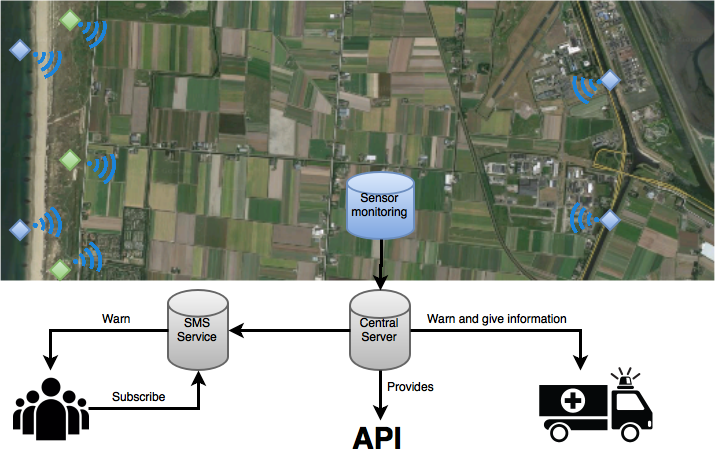
\includegraphics[keepaspectratio=true,width=0.9\textwidth]{images/archVision.png}
	\caption{Schematic overview of the flood monitoring system}
	\label{fig:architectural-vision}
\end{figure}
\newglossaryentry{API}{name=API, description={Application Programming Interface}}
\newglossaryentry{UAV}{name=UAV, description={Unmanned Aerial Vehicle}}

The \gls{SFM} system consists of multiple parts. These are represented in figure \ref{fig:architectural-vision}. First of all there is the monitoring part. This part monitors the current state of the environment. To achieve this, a lot of data is needed, which the system obtains using sensors, weather \gls{API}s and \gls{UAV}s. We use sensors to get the current water level of waterways, these water sensors are shown in the figure as blue squares. We also measure the density and structure of dikes, this is done by pressure meters, temperature meters and tilt meters. These are represented as green squares. To see how far a flood has spread the system use UAVs. The UAVs are also used to verify sensor data. The data that is obtained through all sensors will be send to the central server. Here the information will be processed. The system then determines if there is an imminent flood.

In case of an imminent flood a warning will be issued to the safety region and the citizens who live in the threatened area. We do this by issuing a warning to the safety region. In their turn the safety region can use their infrastructure to warn the citizens. Besides this, citizens can also apply for our SMS service. People who are subscribed to this service will receive a text message when a flood is imminent.

If citizens want to have more information on an imminent flood, they can always access the API. This API gives relevant raw data about imminent floods. To make a usable interface for the citizens, cooperation with third party developers is desired. These developers could create an application that can guide citizens to a save area.
%http://www.waterforum.net/Artikel/PrintArtikel.aspx?ID=9132
